\section{Introduction}
\label{sec:intro}

Cervical cancer is among the most preventable malignancies, and prevention rests on cytological
screening of Papanicolaou-stained smears. Because expert cytologists are scarce and manual reading is
slow and observer-dependent, automated cell classification has become an active frontier, and modern
convolutional networks now report accuracies above $0.95$ on public benchmarks such as
\sipakmed~\cite{plissiti2018sipakmed}. This success has fuelled the expectation that screening can be
partially automated. The dominant evaluation paradigm, however, is \emph{single-dataset}: a model is
trained and tested on splits of one collection, prepared under one staining and segmentation
protocol, and the resulting accuracy is reported as if it were an intrinsic property of the model.
This conflates two very different quantities---how well a model fits the statistics of \emph{one}
slide-preparation pipeline, and how well it would generalise to the heterogeneous slides of clinical
practice. The gap between them is exactly where a deployable screening tool succeeds or fails, and it
is rarely measured.

\begin{figure*}[t]
  \centering
  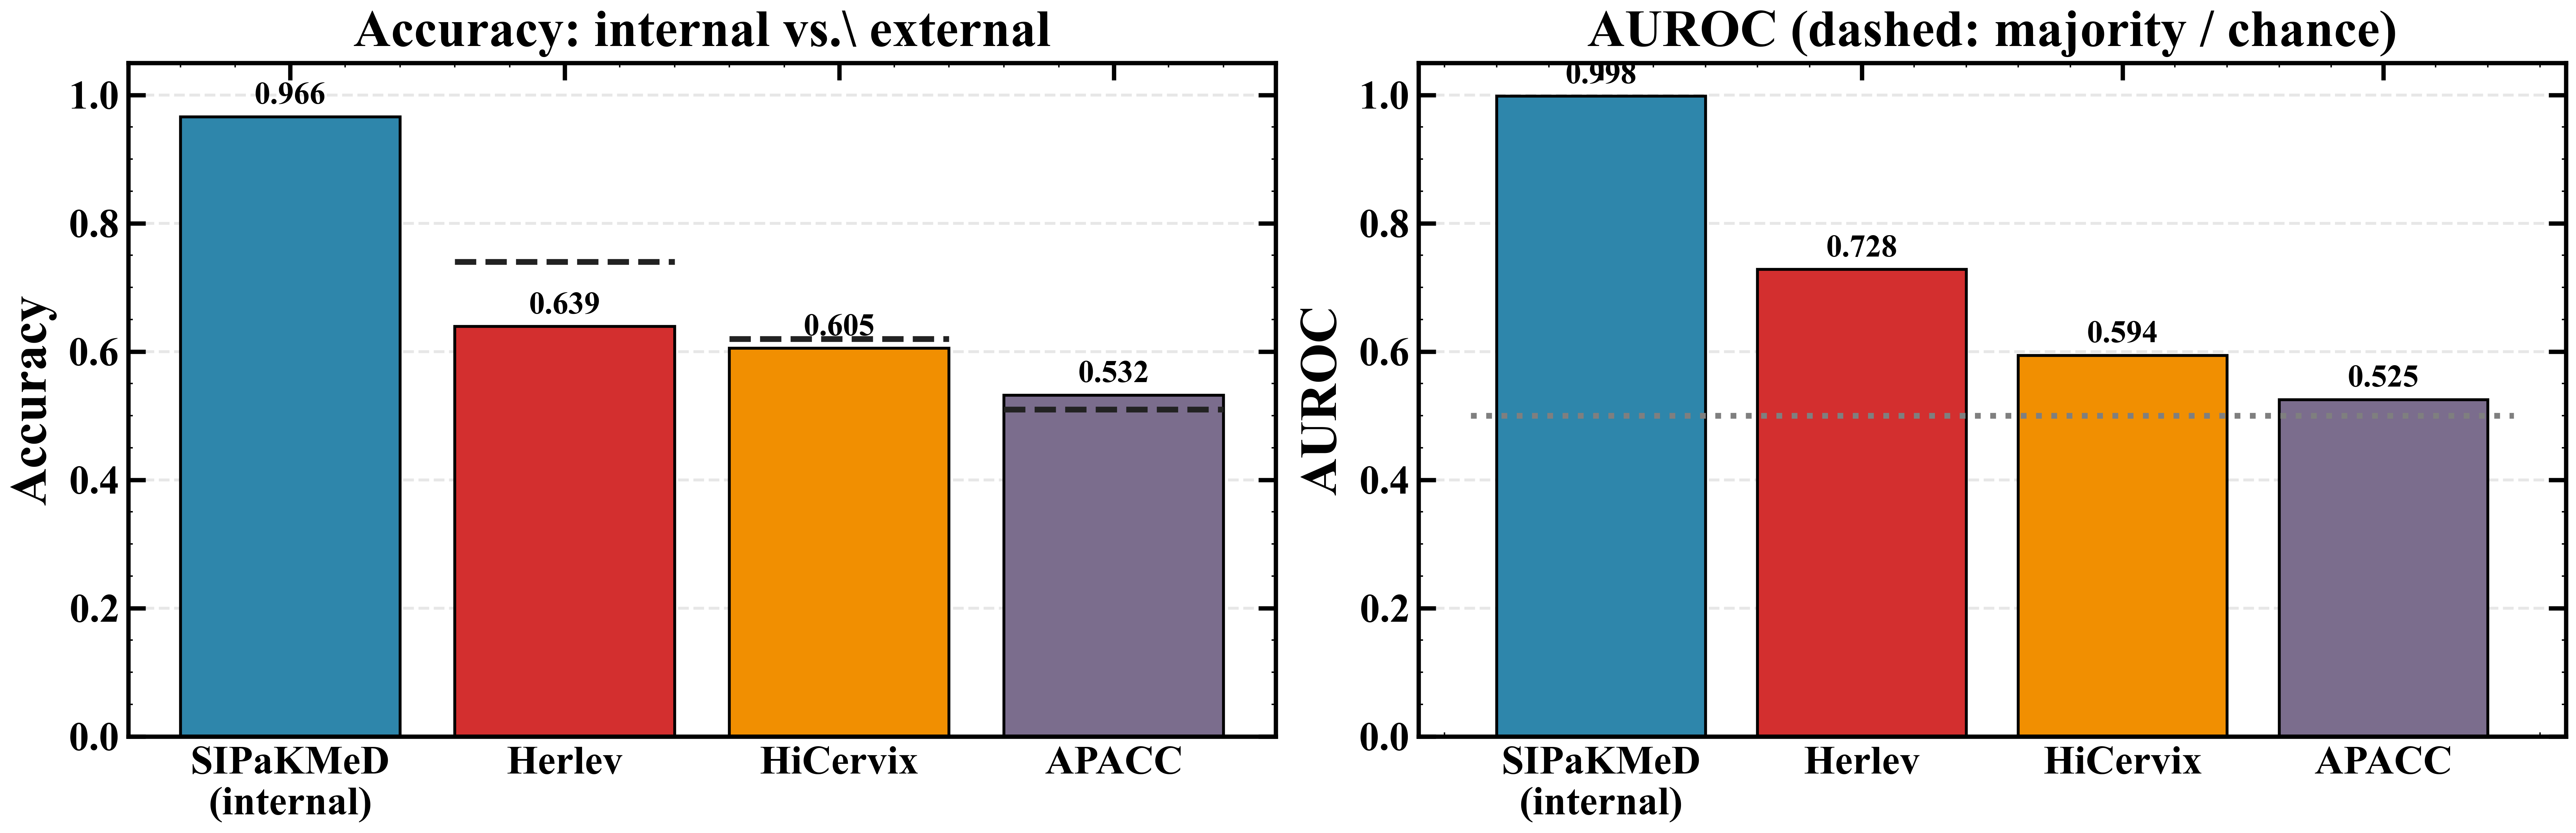
\includegraphics[width=0.92\textwidth]{teaser.png}
  \caption{\textbf{Internal excellence, external collapse.} The distilled student is excellent
  \emph{within} \sipakmed\ (accuracy $0.966$, AUROC $0.998$) but, evaluated unchanged on three
  external Papanicolaou datasets under a binary Normal/Abnormal alignment, collapses to
  $0.53\!-\!0.64$ accuracy and $0.53\!-\!0.73$ AUROC. Dashed lines mark the per-dataset majority-class
  baseline (left) and chance (right): at a fixed threshold the model falls \emph{below} the trivial
  baseline on two of three datasets despite retaining above-chance ranking signal. Severity tracks
  slide-preparation distance from \sipakmed's conventional smear.}
  \label{fig:teaser}
\end{figure*}

We subject a representative high-accuracy system to exactly such a measurement. We study a
knowledge-distilled classifier~\cite{hinton2015distilling} in which an EfficientNet-B4
teacher~\cite{tan2019efficientnet}, ImageNet-pretrained~\cite{deng2009imagenet} and trained on the
five \sipakmed\ cytomorphology classes, is distilled into a compact EfficientNet-B0 student. The
student is attractive for deployment---$4.67$\,M parameters against the teacher's $18.5$\,M---and we
ask whether such compression sacrifices accuracy, calibration, explainability, or generalisation. We
then evaluate the \emph{same} student, without retraining, across three independent Papanicolaou
datasets---\herlev~\cite{jantzen2005herlev}, \apacc, and \hicervix~\cite{cai2024hicervix}---that
differ in staining, segmentation and slide preparation (conventional smear, auto-segmented crops, and
liquid-based cytology). Because the five \sipakmed\ morphology classes do not share a label space
with the dysplasia and Bethesda~\cite{nayar2015bethesda} schemes of those datasets, we align them at
the only common, deterministically mappable level---a binary Normal-versus-Abnormal decision---with
glandular and out-of-scope categories explicitly excluded and the excluded fraction reported.

In-distribution the model is genuinely strong: the distilled student reaches accuracy $0.966$ and
\emph{exceeds its teacher on every metric}, is well calibrated (ECE\,$0.015$), and produces
cytologically plausible Grad-CAM~\cite{selvaraju2017gradcam} attributions. Out-of-distribution it
\emph{collapses} (\cref{fig:teaser}): binary accuracy falls to $0.639$ (\herlev), $0.605$ (\hicervix)
and $0.532$ (\apacc)---below the majority baseline on two of three sets---and AUROC to $0.73$, $0.59$,
$0.53$. The central scientific question is then \emph{why}, and in particular whether the failure is
a labelling/mapping artefact or a genuine model failure. We show it is the latter: the $\pabn$ score
ranks abnormal above normal cells in \emph{every} dataset (all AUROC$>0.5$), so the mapping is
correctly oriented; the collapse is genuine domain shift compounded by an operating-point
miscalibration that does not transfer across domains~\cite{guo2017calibration}, the cytology analogue
of shortcut learning~\cite{geirhos2020shortcut}. We make four contributions.

\begin{itemize}[leftmargin=1.2em,itemsep=1pt,topsep=2pt]
\item \textbf{C1 (a failure mode, characterised).} A reproducible cross-dataset audit showing that a
high-accuracy, well-calibrated, explainable distilled cytology model collapses on three independent
Pap datasets---below the majority baseline at a fixed threshold (\cref{sec:analysis}).
\item \textbf{C2 (a diagnosis, not just a number).} A methodology that mechanistically separates a
labelling artefact from genuine domain failure via class-conditional $\pabn$ separation, an
AUROC-above-chance test, and an accuracy-versus-majority-baseline / oracle-threshold analysis;
applied here it rules out relabelling and isolates domain shift $+$ operating-point miscalibration
(\cref{sec:analysis}).
\item \textbf{C3 (distillation paradox).} Evidence that distillation yields a \emph{smaller-yet-stronger}
in-distribution model---the B0 student surpasses its B4 teacher on every metric---which nonetheless
fails out-of-distribution, decoupling compression quality from generalisation (\cref{sec:exp}).
\item \textbf{C4 (honest evaluation).} We show the internal $0.966$ is itself optimistic
(same-field-of-view leakage), and give evidence-led remedies: leakage-safe cluster-grouped splits,
stain/domain normalisation~\cite{macenko2009stain}, per-domain calibration, and reporting
threshold-free AUROC with the excluded fraction (\cref{sec:discussion}).
\end{itemize}

\noindent\textbf{Paper organisation.} \Cref{sec:questions} states the research questions, hypotheses
and novelty; \cref{sec:primer} fixes cytology background and notation; \cref{sec:related} reviews
related work; \cref{sec:problem} defines the datasets and label alignment; \cref{sec:method} details
the data and training pipeline; \cref{sec:exp} reports in-distribution results; \cref{sec:analysis}
presents the cross-dataset collapse and its diagnosis; \cref{sec:discussion} discusses scope and
remedies.
